%!TEX program = xelatex
\documentclass[11pt, a4paper]{article}
  \usepackage[a4paper,top=3cm,bottom=4cm,left=2.5cm,right=2.5cm]{geometry}
  \usepackage{subfig}
  \usepackage{graphicx}
  \graphicspath{{../images/}}
  \usepackage{hyperref}
  \usepackage{amsmath}
  \usepackage{enumitem}
  \usepackage{mathtools}
  \usepackage{xepersian}
  \settextfont[Scale=1.2]{B Nazanin}
  \setlatintextfont[Scale=1]{Times New Roman Cyr}
  \title{\textbf{شبیه‌سازی رایانه‌ای در فیزیک}\\تمرین سوم: تراوش}
  \author{سینا معمر ۹۵۱۰۲۳۱۶}
    

\begin{document}

\maketitle
\thispagestyle{empty}


\section{\textbf{تراوش}}
کد این بخش از تمرین را در فایل
\lr{q1.py}
می‌توان مشاهده‌ نمود.
در ابتدا لازم است که یک
\lr{object}
از کلاس
\lr{Percolation}
به طول دل‌خواه بسازیم.
سپس تابع
\lr{render}
را با مقدار احتمال موردنظر صدا می‌کنیم.
روش کار این تابع به این صورت است که یک آرایه دو بعدی از اعداد تصادفی به طول داده شده می‌سازد.
سپس این آرایه را با احتمال داده شده مقایسه می‌کند و خانه‌هایی که احتمال کم‌تر داشته باشند را روشن می‌کند.
در آخر نیز برای نمایش، تابع
\lr{show}
را فراخوانی می‌کنیم و با استفاده از تابع
\lr{pcolormesh}
آرایه دو بعدی‌مان را نمایش می‌دهیم.
\\
شکل به دست آمده برای شبکه‌ای به طول
$100$
و احتمال‌های 
$0.4$
و
$0.9$
را در شکل‌های
\ref{fig:q1_100_.4}
و
\ref{fig:q1_100_.9}
می‌توان مشاهده نمود.
همان‌طور که دیده می‌شود برای احتمال
$0.9$
تراوش رخ داده است و خوشه‌ی بی نهایت داریم.

\begin{figure}[h]
	\centering
  \begin{minipage}[b]{0.48\textwidth}
    
\includegraphics[width=\textwidth]{q1_100_0.4.png}
    \caption{شبکه‌ی تراوش به طول $100$ و احتمال $0.4$}
    \label{fig:q1_100_.4}
  \end{minipage}
  \hfill
  \begin{minipage}[b]{0.48\textwidth}
    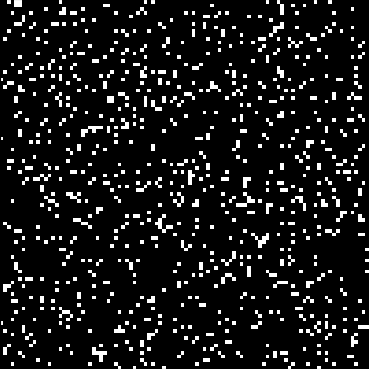
\includegraphics[width=\textwidth]{q1_100_0.9}
    \caption{شبکه‌ی تراوش به طول $100$ و احتمال $0.9$}
    \label{fig:q1_100_.9}
  \end{minipage}
\end{figure}


\section{\textbf{الگوریتم هشن-کپلمن}}
کد این بخش از تمرین را در فایل
\lr{q2.py}
می‌توان مشاهده نمود.
در ابتدا باید یک
\lr{object}
از کلاس
\lr{Percolation}
بسازیم.
سپس تابع
\lr{render}
را با مقدار احتمال دل‌خواه صدا می‌کنیم.
روش کار این تابع به این صورت است که یک آرایه دو بعدی به طول داده شده از اعداد تصادفی می‌سازد.
سپس آرایه به دست آمده را با احتمال داده شده مقایسه می‌کند و خانه‌هایی که احتمال کم‌تر داشته باشند را روشن می‌کند.
بعد تعداد خانه‌های روشن را می‌شمارد و دو آرایه
\lr{labels}
و
\lr{sizes}
را به آن طول می‌سازد.
سپس روی تمام خانه‌های آرایه‌ی دو بعدی‌مان پیمایش می‌کند و شماره‌ی خانه‌های بالا و چپ را می‌خواند.
حال اگر تنها خانه‌ی بالا و یا چپ خالی باشد،
لیبل آن خانه را به آن می‌دهد.
در صورتی هم که هر دو پر باشند، لیبل خانه‌ی چپ را به هر دو می‌دهد.
ولی باید لیبل نهایی آن خانه را پیدا کند و این کار را با استفاده از تابع
\lr{\_\_find\_label}
انجام می دهد.
روش کار این تابع به این شکل است که مقدار لیبل را از آرایه‌ی
\lr{labels}
به دست می‌آورد. اگر این مقدار برابر با شماره خود لیبل باشد،
که همان مقدار نهایی خواهد بود، در غیر این صورت همین تابع را با مقدار به دست‌ آمده صدا می‌کند،
تا در نهایت به جایی برسد که مقدار لیبل با شماره‌ی خانه یکی شود.
\\
برای پیدا کردن خوشه‌ی بی‌نهایت، لیبل خانه‌های ستون اول و آخر را برای اشتراک چک می‌کنیم.
همین کار را برای خانه‌های ردیف اول و آخر انجام می‌دهیم. در صورت وجود اشتراک، یعنی تراوش رخ داده است.
برای این کار تابع
\lr{infinity\_clusters}
را صدا باید بکنیم. خروجی این تابع لیبل خوشه‌ی بی‌نهایت و اندازه‌ی آن است.
\\
برای پیدا طول هم‌بستگی نیز باید تابع
\lr{correlation\_length}
را صدا بزنیم. 
برای به دست آوردن طول هم‌بستگی، روی خانه‌های آرایه‌مان پیمایش می‌کنیم و
‌مختصات خانه‌هایی که لیبل یکسان دارند را در یک آرایه‌ی جدید ذخیره می‌کنیم.
سپس لیبل خوشه‌ی بی‌نهایت را از تابع
\lr{infinity\_clusters}
به دست می‌آوریم و آن را از محاسبات‌مان خارج می‌کنیم.
سپس اندیس بزرگ‌ترین خوشه‌ی باقی مانده را پیدا می‌کنیم و
انحراف معیار مختصات خانه‌های آن لیبل را به دست می‌آوریم و به عنوان خروجی بر می‌گردانیم.
برای نمایش شبکه‌ی تراوش نیز باید تابع
\lr{show}
را فراخوانی کنیم.
\\
نتیجه‌ی به دست آمده برای شبکه‌ای به طول
$100$
و احتمال‌های
$0.4$
و
$0.6$
را در شکل‌های
\ref{fig:q2_100_.4}
و
\ref{fig:q2_100_.6}
می‌توان مشاهده نمود.
همان‌طور که دیده می‌شود، برای احتمال
$0.6$
تراوش رخ داده است.

\begin{figure}[h]
	\centering
  \begin{minipage}[b]{0.48\textwidth}
    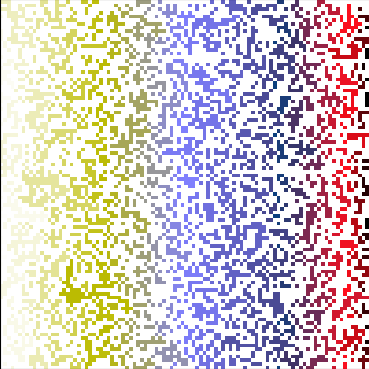
\includegraphics[width=\textwidth]{q2_100_0.4.png}
    \caption{شبکه‌ی تراوش به طول $100$ و احتمال $0.4$}
    \label{fig:q2_100_.4}
  \end{minipage}
  \hfill
  \begin{minipage}[b]{0.48\textwidth}
    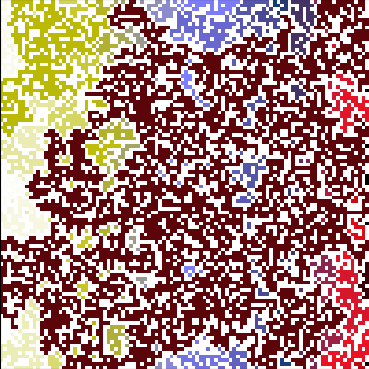
\includegraphics[width=\textwidth]{q2_100_0.6.png}
    \caption{شبکه‌ی تراوش به طول $100$ و احتمال $0.6$}
    \label{fig:q2_100_.6}
  \end{minipage}
\end{figure}


\section{\textbf{احتمال ایجاد خوشه‌ی بی‌نهایت برای شبکه‌ی محدود}}
کد این بخش از تمرین را در فایل
\lr{q3.py}
می‌توان مشاهده نمود.
برای به دست‌ آوردن نتایج خواسته شده تابع
\lr{find\_q}
را باید صدا بزنیم.
روش کار این تابع به این صورت است که روی طول‌های داده شده و سپس روی احتمال‌های داده شده،
پیمایش می‌کند و
\lr{object}
ساخته شده از کلاس
\lr{Percolation}
را با آن طول و احتمال به اندازه تعداد نمونه‌های خواسته شده، صدا می‌کند.
سپس تابع
\lr{is\_percolated}
را فراخوانی می‌کند و در صورتی که تراوش رخ داده باشد، خانه‌ی متناظر با آن در آرایه‌ی داده‌ها را
$1$
می‌کند.
نتایج به دست آمده در یک آرایه ذخیره می‌شوند و آن را در نهایت در یک فایل به فرمت
\lr{.npy}
برای استفاده‌های بعدی ذخیره می‌کند.
سپس میانگین و انحراف معیار داده‌های به دست آمده را محاسبه و رسم می‌کنیم.
نتیجه‌ی به دست آمده را در شکل
\ref{fig:q3_0.05_100_(10, 100, 200)}
می‌توان مشاهده نمود.

\begin{figure}[h]
  \centering
  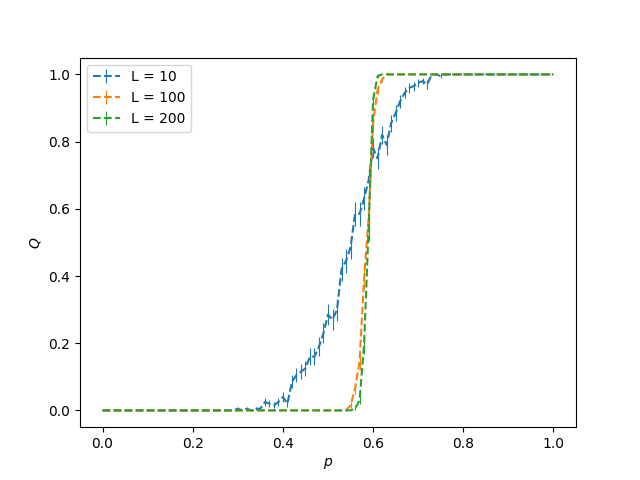
\includegraphics[width=.7\textwidth]{q3_0.01_200_(10, 100, 200)}
  \caption{احتمال تراوش بر حسب $p$  برای شبکه‌هایی به طول $10$، $100$ و $200$ و با $200$ بار تکرار}
  \label{fig:q3_0.05_100_(10, 100, 200)}
\end{figure}


\section{\textbf{احتمال اتصال به خوشه‌ی بی‌نهایت}}
کد این بخش از تمرین را در فایل
\lr{q4.py}
می‌توان مشاهده نمود.
برای به دست‌ آوردن نتایج خواسته شده تابع
\lr{find\_q\_inf}
را باید صدا بزنیم.
روش کار این تابع به این صورت است که روی طول‌ها و سپس روی احتمال‌های داده شده،
پیمایش می‌کند و
\lr{object}
ساخته شده از کلاس
\lr{Percolation}
را با آن طول و احتمال به اندازه‌ی تعداد نمونه‌های خواسته شده، صدا می‌کند.
سپس تابع
\lr{infinity\_clusters}
را فراخوانی می‌کند و در صورتی که تراوش رخ داده باشد،
اندازه خوشه‌ی بینهایت را در خانه‌ی متناظر با آن در آرایه‌ی داده‌ها را ذخیره می‌کند.
نتایج به دست آمده در یک آرایه ذخیره می‌شوند و آن را در نهایت در یک فایل به فرمت
\lr{.npy}
برای استفاده‌های بعدی ذخیره می‌کنیم.
سپس میانگین و انحراف معیار داده‌های به دست آمده را محاسبه و رسم می‌کنیم.
نتیجه‌ی به دست آمده را در شکل
\ref{fig:q4_0.05_100_(10, 100, 200)}
می‌توان مشاهده نمود.

\begin{figure}[h]
  \centering
  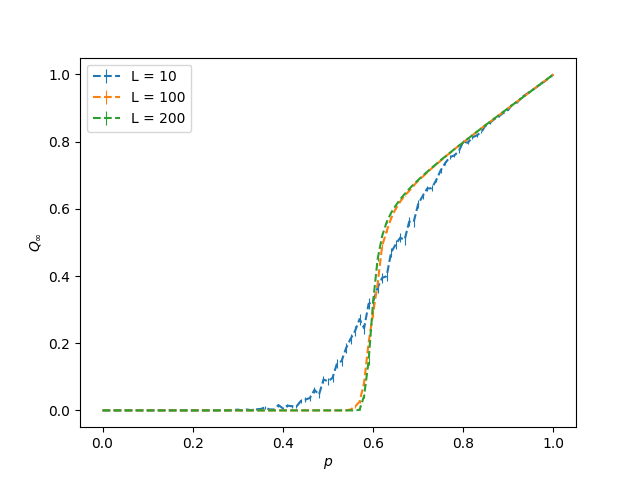
\includegraphics[width=.7\textwidth]{q4_0.01_200_(10, 100, 200).png}
  \caption{احتمال اتصال به خوشه‌ی بی‌نهایت بر حسب $p$ برای شبکه‌هایی به طول $10$، $100$ و $200$ و با $200$ بار تکرار}
  \label{fig:q4_0.05_100_(10, 100, 200)}
\end{figure}


\section{\textbf{طول هم‌بستگی}}
کد این بخش از تمرین را در فایل
\lr{q5.py}
می‌توان مشاهده نمود.
برای به دست‌ آوردن نتایج خواسته شده تابع
\lr{find\_correlation\_radius}
را باید صدا بزنیم.
روش کار این تابع به این صورت است که روی طول‌ها و سپس روی احتمال‌های داده شده،
پیمایش می‌کند و
\lr{object}
ساخته شده از کلاس
\lr{Percolation}
را با آن طول و احتمال به تعداد نمونه‌های خواسته شده، صدا می‌کند.
سپس تابع
\lr{correlation\_length}
را فراخوانی می‌کند و مقدار به دست آمده را در خانه‌ی متناظر با آن در آرایه‌ی داده‌ها ذخیره می‌کند.
نتایج به دست آمده در یک آرایه ذخیره می‌شوند و آن را در نهایت در یک فایل به فرمت
\lr{.npy}
برای استفاده‌های بعدی ذخیره می‌کنیم.
سپس میانگین و انحراف معیار داده‌های به دست آمده را محاسبه و رسم می‌کنیم.
نتیجه‌ی به دست آمده را در شکل
\ref{fig:q5_(10, 20, 40, 80, 160)}
می‌توان مشاهده نمود.
\\
همان‌طور که در شکل دیده می‌شود، قله‌ی منحنی‌ها در حدود بازه‌ی
$(0.5, 0.6)$
قرار دارند.
برای اینکه بتوانیم مقدار
$p_c$
را برای هر کدام با دقت تعیین کنیم، برای هر طول در یک بازه‌ی محدود
و با گام‌های کوچک و تعداد نمونه‌های زیاد، محاسبات قبلی را تکرار می‌کنیم.
نتایج به دست آمده را در شکل‌های
\ref{fig:q5_10}
تا
\ref{fig:q5_160}
می‌توان مشاهده نمود.
مقدار
$p_c$
های به دست‌ آمده از روی این نمودار‌ها در جدول
\ref{tab:p_c_l}
ثبت شده است.

\begin{table}[h]
  \centering
  \begin{tabular}{|c|c|c|c|c|c|}
    \hline
    $160$ & $80$ & $40$ & $20$ & $10$ & طول شبکه \\
     \hline
    $0.581$ & $0.573$ & $0.563$ & $0.539$ & $0.497$ & $p_c \pm 0.001$ \\
     \hline
  \end{tabular}
  \caption{$p_c$ بر حسب طول شبکه}
  \label{tab:p_c_l}
\end{table}

برای به دست آوردن
$p_c(\infty)$
از طریق برون‌یابی مقادیر به دست آمده برای طول‌های محدود،
می توان از رابطه‌ی
\eqref{eqn:p_infty}
استفاده نمود.
در این رابطه
$3$
پارامتر
$A$،
$\nu$
و
$p_c(\infty)$
مجهول هستند.
پس تابع مدل آن‌ها را می‌سازیم و با استفاده از تابع
\lr{curve\_fit}
از کتاب‌خانه
\lr{scipy}
بهترین مقدار آن‌ها را حساب می‌کنیم.
مقدار به دست آمده برای 
$p_c(\infty)$
برابر است با:

\begin{equation}
  p_c(\infty) = 0.5932 \pm 10^{-4}
\end{equation}

\begin{align}
  & |p_c(L) - p_c(\infty)| \sim L^{-\frac{1}{\nu}} \nonumber \\
  & \Rightarrow
  L^{-\frac{1}{\nu}} = A|p_c(L) - p_c(\infty)| \nonumber \\
  & \Rightarrow
  L = (A |p_c(L) - p_c(\infty)|)^{-\nu}
  \label{eqn:p_infty}
\end{align}

\begin{figure}[h]
  \centering
  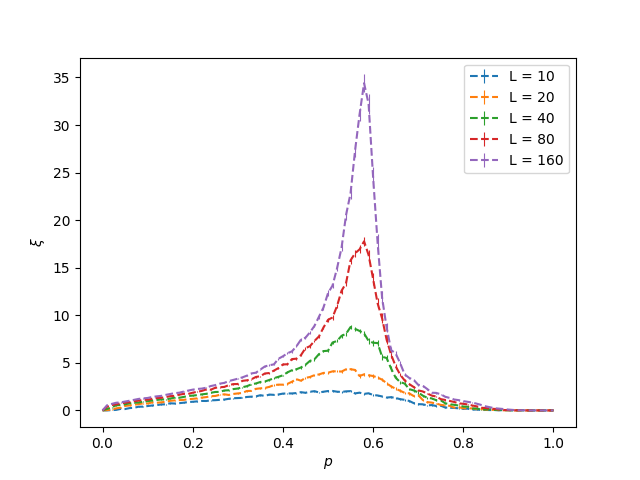
\includegraphics[width=.7\textwidth]{q5_0.0_0.01_1.0_100_(10, 20, 40, 80, 160).png}
  \caption{طول هم‌بستگی بر حسب $p$ برای طول‌های $10$، $20$، $40$، $80$ و $160$ و با $200$ بار تکرار}
  \label{fig:q5_(10, 20, 40, 80, 160)}
\end{figure}

\begin{figure}[h]
	\centering
  \begin{minipage}[b]{0.48\textwidth}
    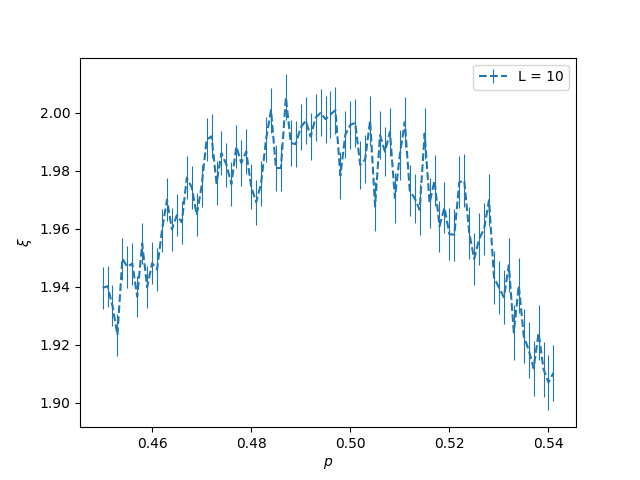
\includegraphics[width=\textwidth]{q5_0.45_0.001_0.54_6000_(10,)}
    \caption{طول هم‌بستگی بر حسب $p$ برای طول $10$ و گام $0.001$ و با $6000$ بار تکرار}
    \label{fig:q5_10}
  \end{minipage}
  \hfill
  \begin{minipage}[b]{0.48\textwidth}
    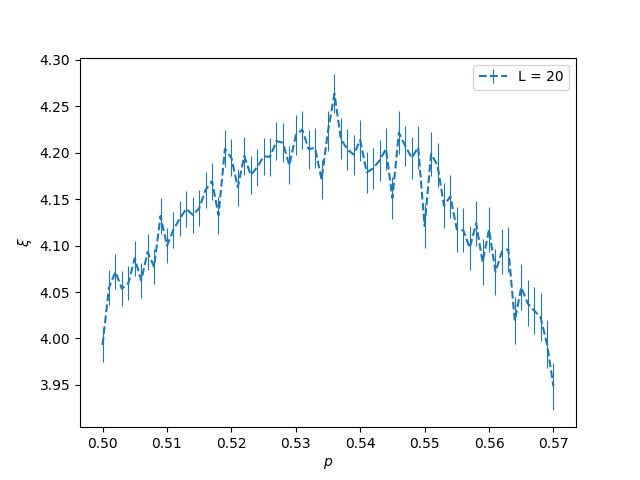
\includegraphics[width=\textwidth]{q5_0.5_0.001_0.57_3000_(20,)}
    \caption{طول هم‌بستگی بر حسب $p$ برای طول $20$ و گام $0.001$ و با $3000$ بار تکرار}
    \label{fig:q5_20}
  \end{minipage}
  \begin{minipage}[b]{0.48\textwidth}
    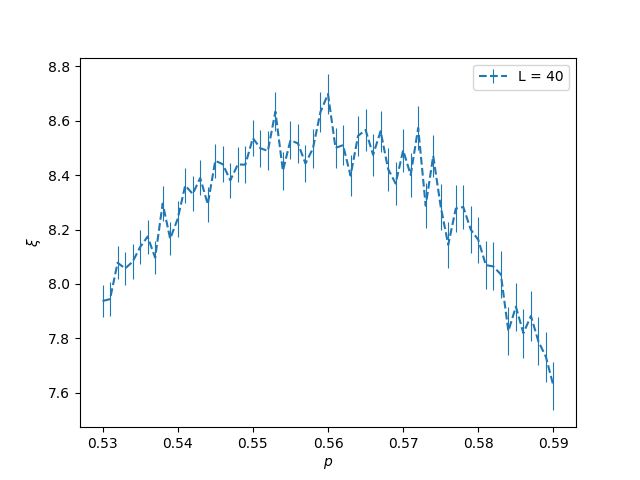
\includegraphics[width=\textwidth]{q5_0.53_0.001_0.59_1000_(40,)}
    \caption{طول هم‌بستگی بر حسب $p$ برای طول $40$ و گام $0.001$ و با $1000$ بار تکرار}
    \label{fig:q5_40}
  \end{minipage}
  \hfill
  \begin{minipage}[b]{0.48\textwidth}
    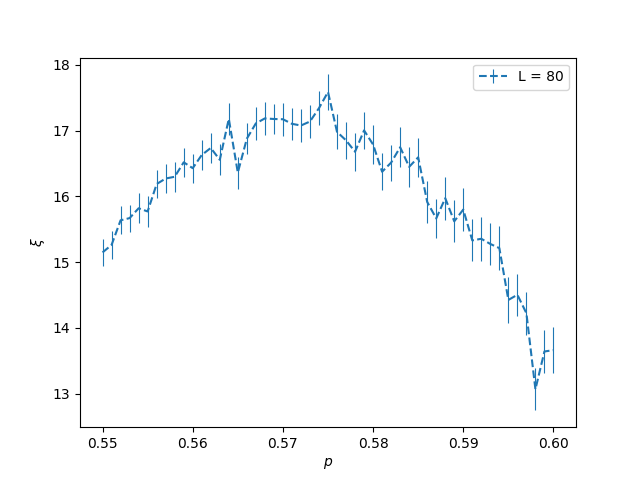
\includegraphics[width=\textwidth]{q5_0.55_0.001_0.6_300_(80,)}
    \caption{طول هم‌بستگی بر حسب $p$ برای طول $80$ و گام $0.001$ و با $300$ بار تکرار}
    \label{fig:q5_80}
  \end{minipage}
  \begin{minipage}[b]{0.48\textwidth}
    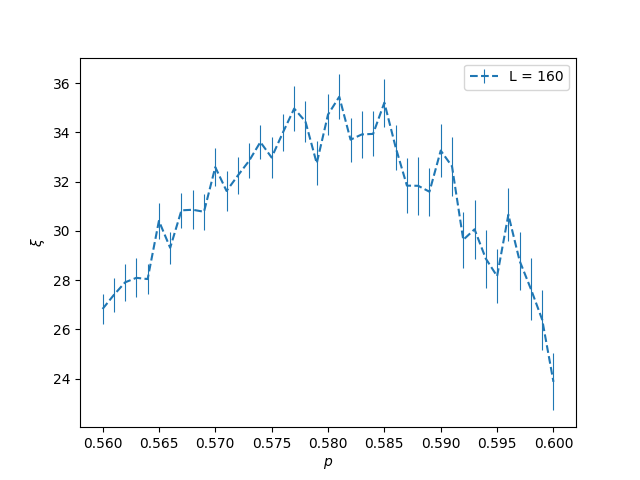
\includegraphics[width=\textwidth]{q5_0.56_0.001_0.6_100_(160,)}
    \caption{طول هم‌بستگی بر حسب $p$ برای طول $160$ و گام $0.001$ و با $100$ بار تکرار}
    \label{fig:q5_160}
  \end{minipage}
\end{figure}


\section{\textbf{نمای بحرانی $\nu$}}
کد این بخش از تمرین را در فایل
\lr{q6.py}
می‌توان مشاهده نمود.
همان‌طور که از رابطه‌ی
\eqref{eqn:q_6_p_l}
دیده می‌شود، با رسم منحنی‌
$|p_c(L) - p_c(\infty)|$
بر حسب
$L$
به صورت تمام لگاریتم، می‌توانیم از روی شیب خط فیت شده، مقدار نمای
$\nu$
را به دست بیاوریم. نمودار به دست آمده را در شکل
\ref{fig:q6_nu}
می‌توان مشاهده نمود. مقدار حاصل برابر است با:

\begin{equation}
  \nu = 1.331 \pm 0.001
\end{equation}

\begin{figure}[h]
  \centering
  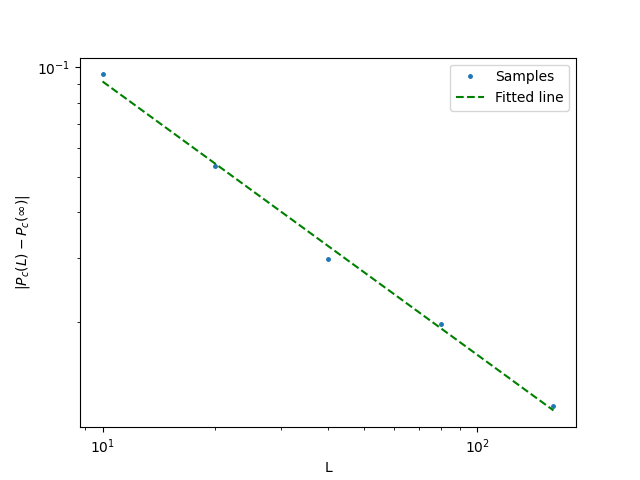
\includegraphics[width=.7\textwidth]{q6_[10, 20, 40, 80, 160]_width.png}
  \caption{$|p_c(L) - p_c(\infty)|$ بر حسب طول شبکه برای طول‌های $10$، $20$، $40$، $80$ و $160$}
  \label{fig:q6_nu}
\end{figure}

\begin{align}
  & |p_c(L) - p_c(\infty)| \sim L^{-\frac{1}{\nu}} \nonumber \\
  & \Rightarrow \ln(|p_c(L) - p_c(\infty)|) = A - \frac{1}{\nu} \ln(L)
  \label{eqn:q_6_p_l}
\end{align}


\section{\textbf{بعد جرمی (فراکتالی) خوشه‌های بی‌نهایت}}
کد این بخش از تمرین را در فایل
\lr{q7.py}
می‌توان مشاهده نمود.
در ابتدا باید یک
\lr{object}
از کلاس
\lr{Percolation}
با طول دل‌خواه بسازیم.
سپس تابع
\lr{render}
را با احتمال موردنظر فراخوانی می‌کنیم.
شیوه‌ی کار این تابع به این صورت است که ابتدا یک آرایه‌ی دو بعدی به طول داده شده می‌سازد.
سپس آرایه‌ی
\lr{active\_cells}
را ایجاد می‌کند و مختصات خانه‌ی مرکزی شبکه را به آن اضافه می‌کند.
وظیفه‌ی این آرایه آن است که مختصات خانه‌های جدیدی که در هر مرحله روشن می‌شوند را در خود نگه دارد.
پس تا زمانی که طول این آرایه غیر صفر باشد، باید به رشد دادن خوشه ادامه دهد.
در هر مرحله‌ی رشد، روی تمام خانه‌های آرایه‌ی
\lr{active\_cells}
پیمایش می‌کند و همسایه‌های آن‌ها را در یک آرایه‌ی جدید ذخیره می‌کند.
از آن جایی که این همسایه‌ها می‌توانند اشتراک داشته باشند، در انتها آن‌ها را یکتا می‌کند.
سپس با توجه به احتمال داده شده، این همسایه‌ها را روشن می‌کند و باقی را غیرفعال می‌کند.
در آخر نیز آرایه‌ی
\lr{active\_cells}
را برابر با لیست همسایه‌های جدید روشن قرار می‌دهد.
\\
برای انجام محاسبات خواسته شده در سوال، باید تابع
\lr{calc\_size\_radius}
را صدا بزنیم.
در ابتدا برای شبکه‌ای به طول
$100$
و با احتمال‌های
$0.5$،
$0.55$
و
$0.59$
خوشه‌‌ها را تولید می‌کنیم و نمایش می‌دهیم.
شبکه‌های به دست آمده را در شکل‌های
\ref{fig:q7_100_0.5}،
\ref{fig:q7_100_0.55}
و
\ref{fig:q7_100_0.59}
می‌توان مشاهده نمود.
\\
سپس برای احتمال‌های
$0.5$
تا
$0.59$
و با گام‌های
$0.1$
طول هم‌بستگی و اندازه‌ی خوشه را به دست می‌آوریم و آن‌ها را در خانه‌ی متناظر با آرایه‌ی داده‌مان ذخیره می‌کنیم.
در نهایت نیز این آرایه را در یک فایل با فرمت
\lr{.npy}
برای استفاده‌های بعدی ذخیره می‌کنیم.
سپس میانگین و انحراف معیار داده‌ها را محاسبه کرده و منحنی‌های
\ref{fig:q7_size}،
\ref{fig:q7_radii}
و
\ref{fig:q7_size_radii}
را رسم می‌کنیم.
\\
همان‌طور که در شکل
\ref{fig:q7_size_radii}
دیده می‌شود، می‌توان یک خط بر داده‌های به دست آمده، فیت کرد.
شیب این خط برابر است با بعد جرمی خوشه‌ی تراوش:

\begin{equation}
  D = 1.9801 \pm 10^{-4}
\end{equation}

\begin{figure}[h]
	\centering
  \begin{minipage}[b]{0.3\textwidth}
    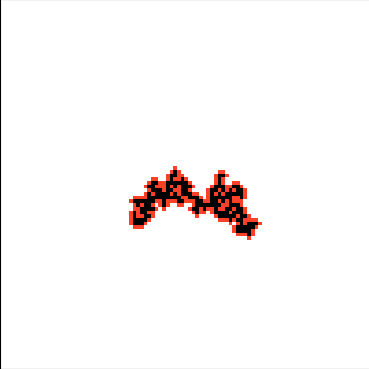
\includegraphics[width=\textwidth]{q7_100_0.5}
    \caption{خوشه‌ی تراوش برای شبکه‌ای به طول $100$ و احتمال $0.50$}
    \label{fig:q7_100_0.5}
  \end{minipage}
  \hfill
  \begin{minipage}[b]{0.3\textwidth}
    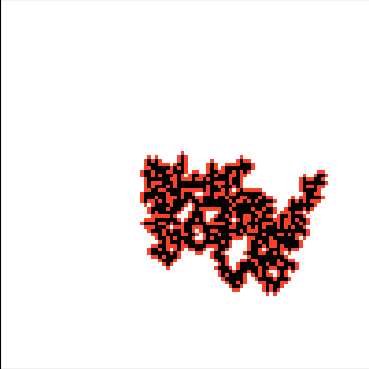
\includegraphics[width=\textwidth]{q7_100_0.55}
    \caption{خوشه‌ی تراوش برای شبکه‌ای به طول $100$ و احتمال $0.55$}
    \label{fig:q7_100_0.55}
  \end{minipage}
  \hfill
  \begin{minipage}[b]{0.3\textwidth}
    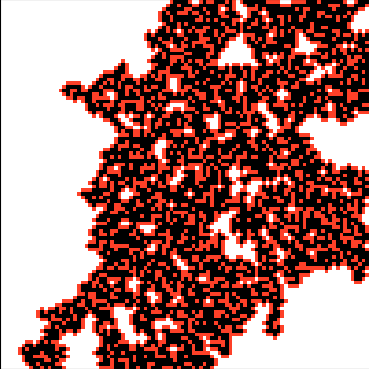
\includegraphics[width=\textwidth]{q7_100_0.59}
    \caption{خوشه‌ی تراوش برای شبکه‌ای به طول $100$ و احتمال $0.59$}
    \label{fig:q7_100_0.59}
  \end{minipage}
\end{figure}

\begin{figure}[h]
	\centering
  \begin{minipage}[b]{0.48\textwidth}
    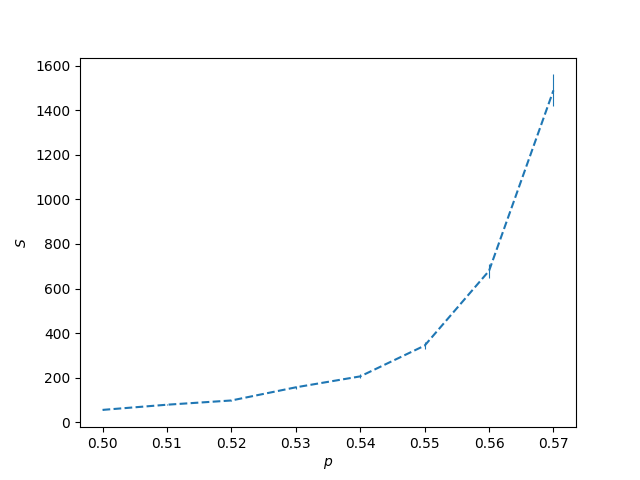
\includegraphics[width=\textwidth]{q7_sizes_0.5_0.01_0.58_1000_10000.png}
    \caption{منحنی اندازه‌ی خوشه بر حسب $p$ برای شبکه‌ای به طول $10\,000$ و با $1000$ بار تکرار}
    \label{fig:q7_size}
  \end{minipage}
  \hfill
  \begin{minipage}[b]{0.48\textwidth}
    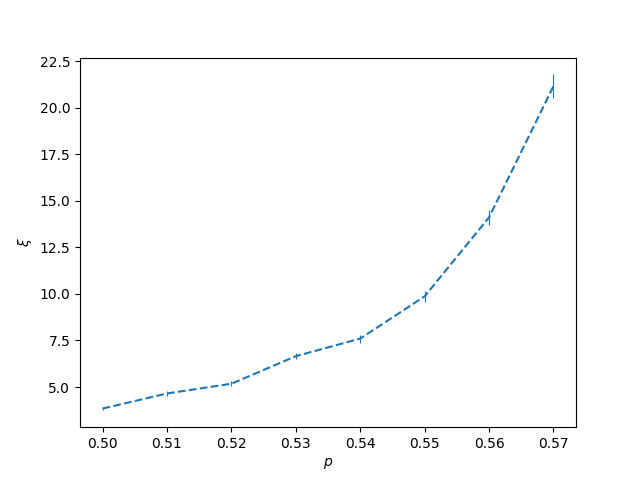
\includegraphics[width=\textwidth]{q7_radii_0.5_0.01_0.58_1000_10000.png}
    \caption{منحنی طول هم‌بستگی خوشه بر حسب $p$ برای شبکه‌ای به طول $10\,000$ و با $1000$ بار تکرار}
    \label{fig:q7_radii}
  \end{minipage}
\end{figure}

\begin{figure}[h!]
  \centering
  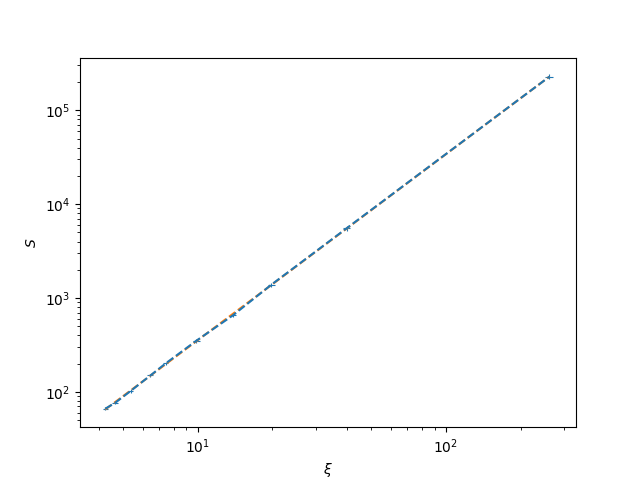
\includegraphics[width=.7\textwidth]{q7_size_radii_0.5_0.01_0.6_1000_10000}
  \caption{منحنی اندازه‌ی خوشه بر حسب طول هم‌بستگی برای شبکه‌ای به طول $10\,000$ و و با $1000$ بار تکرار}
  \label{fig:q7_size_radii}
\end{figure}

\end{document}
